\chapter{What Exactly Is a Gene?}

\begin{kaichang}
Find a family photograph and an advertisement for ``genetic testing,'' handed out on the street or seen on your phone. Familiar terms promise tests for ``athletic genes,'' ``obesity genes,'' ``talent genes,'' ``alcohol-metabolism genes,'' and ``baldness genes.'' In the photo, your eyes resemble your father's and your face your mother's, while some features resemble neither.

Without looking anything up, guess what someone means by ``testing one of your genes.'' Will they measure a protein's concentration, count chromosomes, or find a short passage in your three-billion-letter DNA scroll and read its letters?

``Gene'' may be modern science's most-used and vaguest word. Advertisements and news use it; relatives use it when saying a talented child ``takes after Dad---good genes.'' Yet ask what a gene physically is, and few can answer. This chapter will. At the end, we return to the advertisement and decode ``testing a gene.''

Consider everyday phrases: ``His athletic talent comes from good genes,'' ``This condition is inherited,'' ``Can we eat genetically modified food?'' and ``Police identified a suspect through DNA.'' Their ``genes'' belong to different levels: a trait, disease susceptibility, an artificially transferred sequence, and letter differences used for identification. A word serving so many users and purposes almost inevitably blurs. Our aim is not another definition to memorize, but to take the gene apart until its components become visible.
\end{kaichang}

\section{Everyone Says Gene; Where Is It?}

Start with what is visible. You resemble your parents without matching them. Peas have purple or white flowers and round or wrinkled seeds (Chapter 63). Kittens in one litter differ in coat color. Ancient people already knew that ``melons produce melons.'' Yet resemblance itself is difficult to pin down, like a mist over every family that everyone feels but nobody can grasp.

Mendel's greatness was turning that mist into countable things. Instead of the impossibly broad ``why do children resemble parents?'' he chose sharply distinct pea traits: purple or white flowers, round or wrinkled seeds. Then he counted hybrid offspring and their ratios (Chapter 63). Counting dispersed the mist to reveal orderly mathematics. He inferred hereditary factors, one pair per trait, one from each parent.

Remember: Mendel never saw a factor. He knew neither whether it was a molecule nor where it lived in cells. He had only an abstraction: \textbf{a trait-controlling unit that can separate and recombine and is transmitted probabilistically}. This first gene definition came entirely from counting. Like Dalton's atoms in Chapter 7, the unit was proposed because it explained measured numbers; its appearance could wait.

You have followed what came later: chromosomes housed the factors (Chapter 64); DNA became hereditary material (65); its helix revealed information in base order (66); replication, transcription, and translation machinery were dissected (67--69); and regulation controlling those messages emerged (70). At this point in the chain, we can finally give the abstract factor a material address.

\section{Zooming onto the DNA Chain}

Imagine a chromosome as an enormous tape densely covered with A, T, G, and C. A human body cell has 46 tapes in 23 pairs, totaling roughly three billion letters, collectively the \textbf{genome}, all your hereditary information. You have two copies of this long collection, paternal and maternal, so most positions have two copies.

Where is a gene? At \textbf{a fixed position} on the scroll, a \textbf{locus}, literally a place or seat. For example, the lactase gene governing lactose digestion occupies a fixed locus on chromosome 2. Everyone has DNA at that position, but letters may differ: your version may differ from your classmate's. Versions at the same locus are \textbf{alleles}. Mendel's dominant and recessive factors in Chapter 63 are alleles at one address. Dominance describes heterozygous expression, never superiority, frequency, or strength.

Fix the relationships clearly:

\begin{itemize}[itemsep=2pt]
\item \textbf{Genome}: the complete scrolls, roughly three billion letters, in two copies.
\item \textbf{Locus}: a fixed position or address on the scrolls.
\item \textbf{Gene}: a sequence at that position capable of producing a functional product.
\item \textbf{Allele}: a version of that sequence at the same position.
\end{itemize}

Notice the third definition differs from Mendel's. His gene was a ``factor controlling a trait''; today's is \textbf{a DNA sequence producing a functional product}. Usually the product is protein, but it can be directly functioning RNA. Why revise the definition? Digging deeper showed that ``controls a trait'' is indirect and misleading. Transcription, translation, protein networks, cells, and a whole body intervene between sequence and trait, the path of Chapter 73. ``Produces a functional product'' can instead be tested directly: what RNA is transcribed, what protein translated, and what does the product do?

Alleles are thoroughly ordinary. Your ABO blood group concerns versions at a chromosome 9 locus encoding a glycosyltransferase. Different enzyme versions attach different sugars to red-cell surfaces. A adds A-type sugar, B adds B-type, while O carries a ``cannot keep reading'' change that disables the enzyme, adding no sugar. Two copies give AA, AO, BB, BO, AB, or OO: six combinations, four blood groups. Dominance here merely means ``adding sugar overrides not adding it''; A and B are equally codominant (Chapter 63). No version is more advanced.

\begin{qiaoliang}
How large is the genome book? A human haploid set has about $3\times 10^{9}$ letters. Print them in this book's type size, about 3000 letters per page:
\[3\times 10^{9} \div 3000 = 10^{6}\ \text{pages}\]
A million pages, or 2000 books of 500 pages, fills a small library. All fits inside a nucleus only about \ud{6}{\mu m} across, through Chapter 66's packaging.
Now calculate the share occupied by genes. Roughly twenty thousand protein-coding genes sound numerous, yet sequences actually translated into protein comprise only about 1.5\% of the genome. Of 2000 books, only thirty are ``main text.'' The rest contains switches, directly functioning RNA sequences, old components, repeated passages, and portions of unknown function. This proportion itself matters: the genome is far from a dictionary of neatly arranged genes.
\end{qiaoliang}

\section{Inside a Gene}

Isolate one gene and magnify its internal structure. A typical eukaryotic gene, including yours, has at least two kinds of region.

First, the \textbf{regulatory region} near its ``front end,'' most famously the promoter (Chapter 68). It encodes no product but provides docking for RNA polymerase and transcription factors, determining where, when, and how loudly a gene is read. Chapter 70's switches and dimmers live here. Regulatory errors can cause disease despite a perfectly normal amino-acid sequence, because the product is made at the wrong time or in the wrong cell. Coding-sequence inspection alone misses that.

Second, the \textbf{transcribed region}, copied into RNA. Its protein-translated portion is the \textbf{coding region}, where codons are read in triplets (Chapter 69). Eukaryotic transcribed regions contain two passage types: \textbf{exons}, joined into final mRNA, and \textbf{introns}, copied but subsequently removed (Chapter 68's splicing). Coding regions assemble from exons separated by potentially many introns. Different splicing can yield several proteins from one gene, another reason ``one gene, one protein'' is historical shorthand.

Here is a schematic assembling these components. Box widths are symbolic, not actual lengths; real introns are often much longer than exons.

\begin{center}
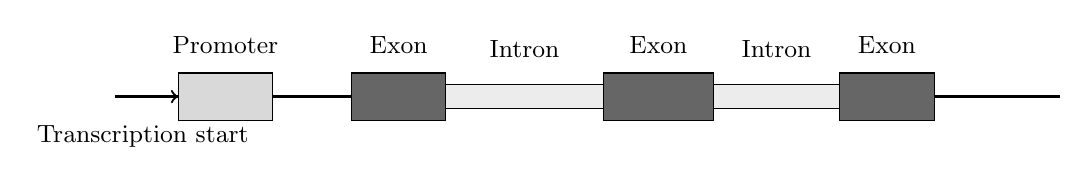
\begin{tikzpicture}[x=1cm,y=1cm]
\draw[thick] (0,0) -- (12,0);
\draw[fill=gray!30] (0.8,-0.3) rectangle (2.0,0.3);
\draw[fill=black!60] (3.0,-0.3) rectangle (4.2,0.3);
\draw[fill=gray!15] (4.2,-0.15) rectangle (6.2,0.15);
\draw[fill=black!60] (6.2,-0.3) rectangle (7.6,0.3);
\draw[fill=gray!15] (7.6,-0.15) rectangle (9.2,0.15);
\draw[fill=black!60] (9.2,-0.3) rectangle (10.4,0.3);
\node at (1.4,0.65) {\small Promoter};
\node at (3.6,0.65) {\small Exon};
\node at (5.2,0.6) {\small Intron};
\node at (6.9,0.65) {\small Exon};
\node at (8.4,0.6) {\small Intron};
\node at (9.8,0.65) {\small Exon};
\draw[->,thick] (0.1,0) -- (0.8,0);
\node at (0.35,-0.5) {\small Transcription start};
\end{tikzpicture}
\end{center}

A gene is therefore not a homogeneous, sharply bounded stretch, but \textbf{a functional region with switches and editing marks}. Whether DNA counts as a gene depends not on length but on whether cells use it to make a useful product and whether it has the corresponding reading controls.

\section{An Experiment Refined the Definition}

``A sequence region producing a functional product'' sounds plain, but generations of experiments refined it. One especially elegant battle involved ``one gene, one enzyme.''

\begin{zhengju}
In the 1940s, Beadle and Tatum studied pink bread mold, Neurospora crassa. Wild type conveniently lives on simple sugar, salts, and one vitamin, making its own amino acids. Their idea was direct: if genes are working instructions, damaging one should disable a specific manufacturing ability.

They irradiated spores with X-rays to induce mutations (Chapter 72), then checked offspring individually on the minimal diet. Most mutants still survived, suggesting the damaged regions were unimportant. A few became ``picky eaters,'' needing an added substance such as arginine. Further tests were revealing: would citrulline work instead? Ornithine? Some mutants survived with ornithine, others required citrulline, and others needed arginine itself. Arginine production must therefore be multistep, with different mutants blocked at different stations. \textbf{Each station corresponded to an enzyme, each enzyme to a damaged gene}. In 1941, they proposed that a gene generally determines an enzyme, later generalized to protein. They received the 1958 Nobel Prize in Physiology or Medicine.

Later work trimmed the rough edges: some proteins assemble products from several genes; some genes produce RNA; alternative splicing generates several proteins from one gene (Chapter 68). Scientific definitions begin with a version useful in battle, then gain precision through evidence. Our opening ``sequence region producing a functional product'' is the current result.
\end{zhengju}

\section{Three Difficult Cases at the Boundary}

Today's definition still has awkward cases. That is no scientific failure: nature does not follow human glossaries. Meet three difficult cases to complete your understanding.

\textbf{Noncoding RNA genes}. Some transcripts work without becoming proteins: tRNA adapts translation, rRNA forms the ribosome's scaffold and catalytic core (Chapter 69), and regulatory RNAs control other genes (Chapter 70). They fit poorly under the old ``trait-controlling factor'' definition, but clearly qualify as functional-product sequences. Their discovery drove the change.

\textbf{Overlapping genes}. Some viruses read one DNA stretch from different starts or in different ways to encode two or three proteins, like changing a sentence's punctuation. Where is one gene's boundary? Overlapping sequences prevent drawing conflict-free divisions on the tape.

\textbf{Pseudogenes}. The genome also carries ``old parts,'' clearly resembling functioning genes but no longer making products after accumulated disruptive changes. Evolution's discarded files sometimes reactivate or provide reusable pieces (Chapter 79 covers duplication, borrowing, and remodeling). Do they count? It depends whether you emphasize products or ancestry.

Biologists therefore use a flexible ruler: \textbf{a sequence region producing a functional product and maintained in evolution}. Context handles blurry cases. Words serve people; nature need not obey them.

\begin{wuqu}
``The genome is a human instruction manual, with every gene a component entry.'' This popular analogy can mislead. No entry directly describes a trait: genes describe protein or RNA products, and all of life intervenes before traits emerge (Chapter 73). Manuals are written to assemble machines, but nobody wrote the genome: billions of years of trial and error accumulated an archive of repeats and discarded files. Most practically, different cells read different content from one genome. Nerve and muscle cells use the same books for different lives (Chapter 70). Think instead of an old kitchen piled with recipes. Recipes do not cook; dishes depend on the cook, the chosen recipe, and the heat.
\end{wuqu}

\section{Genes Work in Networks, Not Isolation}

After locating genes, inspecting their interiors, and refining their definition, add an immediate safeguard: \textbf{one gene almost never determines anything alone}.

Its product immediately enters a network. Lactase matters only when made at the right time in intestinal cells; regulatory regions control its amount (Chapter 70), and folding and transport affect its performance (69). A visible trait---height, skin color, blood group, or milk digestion---often combines many products with environment and experience. Pulling a gene from its network and asking what it determines is like pulling one orchestral musician aside and asking whether they performed the whole symphony.

This explains why alleles are genetics' actual currency. Most people possess the lactase gene; differences arise from \textbf{versions} at the locus. Some digest lactose throughout life; others turn its intestinal volume down in adulthood (Chapters 70 and 74). A report saying you ``carry a particular type'' means it identified the two versions at a locus. Where do versions originate? Mutation, our next subject.

Another frequent inversion needs correction. Environment and networks are not external interference but part of how genes work. A plant in shade or sun reads the same genes into different growth strategies. Bee larvae fed ordinary nectar become workers; those given royal jelly become queens. Sequence is not the difference, its reading is (Chapter 74 discusses an epigenetic mechanism). Genes define a range of possibilities; environment and regulation select within it. Thinking of genes as a die's possible values and development and environment as the throwing hand is better than ``genes determine everything.''

\begin{shiyan}
Draw your own ``version map.'' Get paper and a pen and do a little family homework:
\begin{enumerate}[itemsep=1pt]
\item List yourself, your father, and your mother, or two elders you spend time with.
\item Choose three visible trait versions: tongue rolling, dimples, and clearly backward-bending final thumb joints. Record yes/no or can/cannot for each person.
\item Draw a three-by-three table and enter each observed version.
\item Observe which versions match one parent and whether any match neither. Who supplied your two copies? Which allele combinations might hide behind yes/no entries? Recessive versions need not appear (Chapter 63).
\end{enumerate}
Safety: Observation only. Tongue rolling is no measure of ability or health, merely a harmless difference. Do not infer parentage from these features; a single trait version cannot answer such questions.
\end{shiyan}

\section{Back to the Advertisement}

Now unpack that flyer. ``Testing your alcohol-metabolism gene'' really means collecting cheek cells, extracting DNA, and reading your two copies at the aldehyde-dehydrogenase locus to identify alleles. If a version lowers enzyme activity, acetaldehyde breaks down slowly and drinking readily causes flushing. The report predicts \textbf{a tendency in chemical reaction rate}, not a verdict on how much you can drink: body weight, sex, drinking habits, and many other factors also affect apparent tolerance.

\textbf{Translator safety note:} Do not test a gene prediction by drinking, or interpret tolerance as protection from harm. Alcohol flushing can signal intolerance and is associated with increased risk of certain cancers; masking the flush does not remove that risk. See \href{https://www.niaaa.nih.gov/publications/alcohol-flush-reaction-does-drinking-alcohol-make-your-face-red}{NIAAA alcohol-flush guidance}.

``Talent genes'' and ``athletic genes'' deserve still greater caution. If a trait reflects many genes plus environment, as almost certainly true (Chapter 73), ``test one gene to determine talent'' exceeds evidence. Ask three questions: which locus is tested? Which product and function does the version affect? What evidence connects that product causally to the advertised talent?

Glance at the family photo again. Each parent supplied a set of scrolls. Most addresses contain the same genes, but many have different versions on the two copies. Resemblance to Dad may reflect a dominant version; resembling neither may reflect two recessive versions meeting (Chapter 63), or a polygenic combination neither parent had. Similarity and difference use the same rules.

\section{Next: Where Do Versions Come From?}

We have repeatedly invoked versions at one address while avoiding their origin. Why is one letter common at a human position and another occasional? If a letter changes, does the product change---for worse, better, or not at all?

The answer is neither mysterious nor romantic: copying makes mistakes, radiation breaks molecules, viruses insert themselves, and excellent cellular repair is not infallible. Chapter 72 examines misunderstood mutation, source of most hereditary diseases and evolution's only raw material.

\begin{tiaozhan}
(Optional.) Picture a locus as an interval on a number line. Each copy is one stretch among three billion letters. If a position averages one copying error per $10^{8}$ gamete DNA copies (Chapter 67's proofreading precision), a gene $3\times 10^{4}$ letters long has probability roughly $3\times 10^{4}\times 10^{-8}=3\times 10^{-4}$ of a new error in a generation, about three in ten thousand. Small though that sounds, across twenty thousand genes each person is born with dozens of new letter differences absent from both parents. Multiply across the population, and almost every possible letter error occurs in someone each generation. ``Will a new version appear?'' is therefore a question of time, never probability. Chapters 72 and 77 pursue the calculation.
\end{tiaozhan}

\section*{Try It Yourself}

\begin{sikaoti}
\item Distinguish genome, locus, gene, and allele in your own words, giving examples outside this chapter. Invented examples, such as a plant flower-color locus, are fine.
\item Compare ``sequence region producing a functional product'' with Mendel's ``factor controlling a trait.'' What improves in the new definition, and why does it still need networks and environment?
\item Draw two loci on a chromosome scroll. At one, show two people's two copies, using different shading for allele versions. Note that this is representation; real DNA has no shading.
\item A mutant mold in Beadle and Tatum's experiment survives with arginine or citrulline, but not ornithine. Which pathway station is broken? (Hint: rescuing substances lie downstream of the broken station.)
\item Why are definitions complicated by overlapping genes and noncoding RNA genes? Which part does each challenge?
\item An advertisement offers to test ``the gene determining mathematical talent.'' Using the three questions above, explain to your family why this exceeds the evidence.
\end{sikaoti}
